\documentclass[10pt, a5paper]{article}
\usepackage[T2A]{fontenc}
\usepackage{ucs}
\usepackage[utf8x]{inputenc}
\usepackage[polish,english,russian]{babel}
\usepackage{hyperref}
\usepackage[inner=2cm,top=1.8cm,outer=2cm,bottom=2.3cm,nohead]{geometry}
\usepackage{listings}
\usepackage{graphicx}
\usepackage{wrapfig}
\usepackage{longtable}
\usepackage{indentfirst}
\frenchspacing
\usepackage{fixltx2e} %text sub- and superscripts
\usepackage{icomma} % коскі ў матэматычным рэжыме
\PreloadUnicodePage{4}

\newcommand{\longpage}{\enlargethispage{\baselineskip}}
\newcommand{\shortpage}{\enlargethispage{-\baselineskip}}

\def\switchlang#1{\expandafter\csname switchlang#1\endcsname}
\def\switchlangbe{
\let\saverefname=\refname%
\def\refname{Літаратура}%
\def\figurename{Іл.}%
}
\def\switchlangen{
\let\saverefname=\refname%
\def\refname{References}%
\def\figurename{Fig.}%
}
\def\switchlangru{
\let\saverefname=\refname%
\let\savefigurename=\figurename%
\def\refname{Литература}%
\def\figurename{Рис.}%
}

\hyphenation{admi-ni-stra-tive}
\hyphenation{ex-pe-ri-ence}
\hyphenation{fle-xi-bi-li-ty}
\hyphenation{Py-thon}
\hyphenation{ma-the-ma-ti-cal}
\hyphenation{re-ported}
\hyphenation{imp-le-menta-tions}
\hyphenation{pro-vides}
\hyphenation{en-gi-neering}
\hyphenation{com-pa-ti-bi-li-ty}
\hyphenation{im-pos-sible}
\hyphenation{desk-top}
\hyphenation{elec-tro-nic}
\hyphenation{com-pa-ny}
\hyphenation{de-ve-lop-ment}
\hyphenation{de-ve-loping}
\hyphenation{de-ve-lop}
\hyphenation{da-ta-ba-se}
\hyphenation{plat-forms}
\hyphenation{or-ga-ni-za-tion}
\hyphenation{pro-gramming}
\hyphenation{in-stru-ments}
\hyphenation{Li-nux}
\hyphenation{en-vi-ron-ment}
\hyphenation{Te-le-pathy}
\hyphenation{Li-nux-ov-ka}

\def\progref!#1!{\texttt{#1}}
\renewcommand{\arraystretch}{2} %Іначай формулы ў матрыцы зліпаюцца з лініямі
\usepackage{array}

\def\interview #1 (#2), #3, #4, #5\par{

\section[#1, #3, #4]{#1, #5}
\def\qname{LVEE}
\def\aname{#1}
\def\q ##1\par{{\noindent \bf \qname: ##1 }\par}
\def\a{{\noindent \bf \aname: } \def\qname{L}\def\aname{#2}}
}

\begin{document}
\title{О создании bartop arcade автомата\footnote{\url{a_sorokin@wargaming.net}, \url{http://lvee.org/ru/abstracts/187}}}
\author{Alexandr Sorokin, Minsk, Belarus}
\maketitle
\begin{abstract}
Experience share of building the bartop arcade cabinet from ground up, based on open source technologies.
\end{abstract}
\subsection*{Введение}

Аркады были очень популярны в 70-80е годы. Для некоторых людей это существенная часть детства/юности. Аркадные игры поражают своей увлекательностью и простотой. Несмотря на то, что современные игры стали реалистичнее, красочнее, и <<онлайновее>>, играть в старые аркады по-прежнему интересно. Аркадный автомат становится центром притяжения в веселой компании или в рабочем офисе. Есть несколько вариантов добыть себе такой автомат:

\begin{figure}[h!]
  \centering
  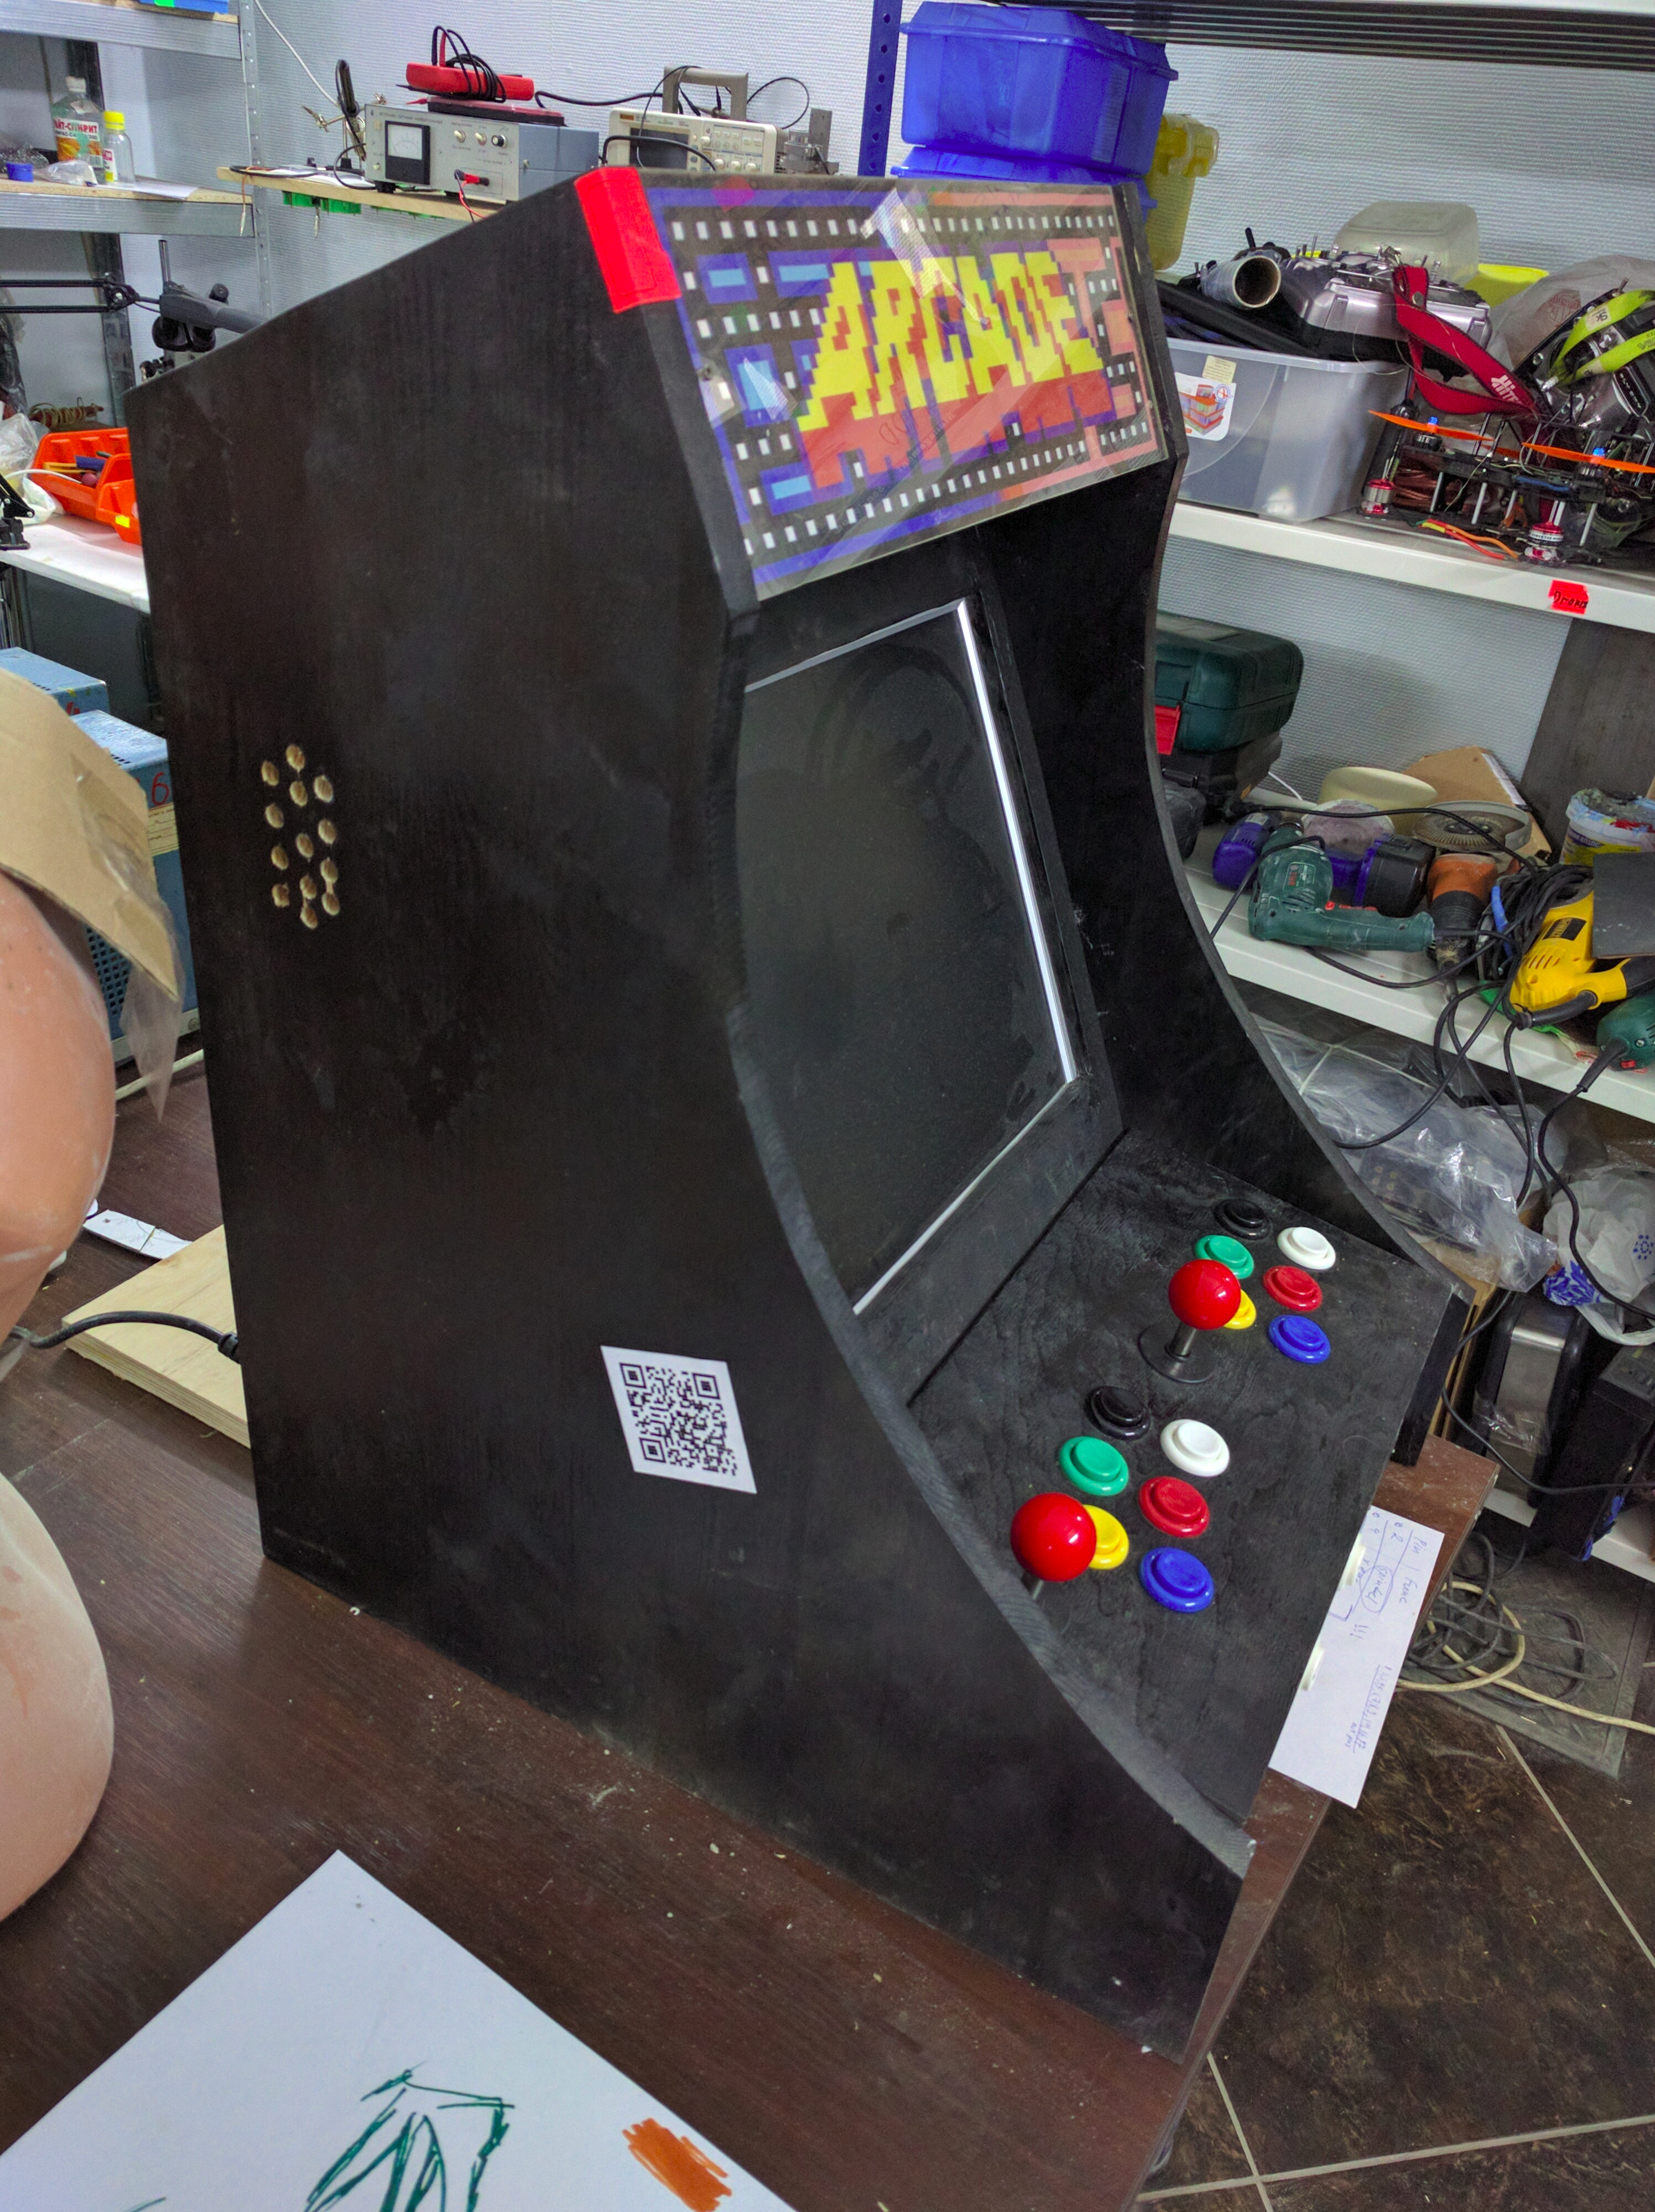
\includegraphics[height=5.7cm]{27_2016_Sorokin1.png}
\end{figure}


\subsection*{Моя история. Начало}

Я выбрал вариант самостоятельной сборки игрового автомата с  нуля. Целью было набить руку в столярном деле, сборке электроники. И, можно отметить, что даже в таком небольшом проекте удалось добить поставленной цели, получив массу опыта.
Начать было нелегко, работа требовала пространства, времени и инструментов. В Минске я узнал о хакерспейсе, который Сложности, мешающие начать работу над проектом, удалось решить благодаря помощи Минского хакерспейса.

\subsection*{Эмуляторы}

Сейчас доступно огромное количество эмуляторов для десятков разнообразных платформ, включая игровые. Весь этот зоопарк эмуляторов организован в системы с фронтендами и даже дистрибутивами.

Наиболее передовые эмуляторы "--- LibRetro и M.A.M.E \linebreak(М.А.М.Е. "--- идеологический отщепенец). Наиболее известные \linebreakфронтенды "--- emulation station, RetroArch, FB Alpha. Популярные дистрибутивы "--- RetroPie, Lakka.

\subsection*{Работа над аппаратом. выбор железа. список покупок}

Существенная доля составных частей аппарата "--- легко доступные материалы и детали. Но также требуется и немного специализированных частей, которые лучше приобрести заранее.
Самое необходимое "--- это набор аркадных кнопок и джойстиков. Все \linebreak остальное более-менее взаимозаменяемо.

\subsection*{Работа над аппаратом. Первые шаги.}

Моделирование корпуса проводилось в OpenScad "--- \linebreak открытом пакете для моделирования путем написания программ на специальном скриптовом языке. Проектирование отталкивалось от идеи, что аппарат должен быть легко разборным, с возможностью заменять отдельные части.
Для начала был изготовлен прототип из картона:

\begin{figure}[h!]
  \centering
  \includegraphics[height=5.7cm]{27_2016_Sorokin2.png}
\end{figure}


Прототип "--- важная стадия проекта, и учет результатов и выводов этого этапа значительно облегчает выполнение последующих этапов.

\subsection*{Работа над аппаратом. Корпус}

Для копруса может быть использован любой легко обрабатываемый материал. Я выбрал клееный деревянный щит для боковин и фанеру 10мм для остальных частей корпуса. 
Удалось сделать разборными части с монитором и консоль с джойстиками, как и планировалось на этапе проектирования.
Тем не менее, был допущен ряд просчетов, которые сказались на внешнем виде аппарата.

\begin{figure}[h!]
  \centering
  \includegraphics[height=5.7cm]{27_2016_Sorokin3.png}
\end{figure}


\subsection*{Работа над аппаратом. Электроника}

Внутри аппарата была необходимость использовать цепи с напряжением 5V и 12V. Изначальной задумкой было использовать интегрированный блок питания на два напряжения. Но в итоге пришлось остановиться на блоке 12V с дополнительным преобразователем DC-DC 12V-5V.

Основной проблемой в части электроники стала аналоговая \linebreak часть, а именно шумы в колонках. Этому было несколько причин.
Проблемы были как с усилителями китайского производства, так и с эффектом ground loop. Последняя проблема решилась только добавлением дополнительного фильтра, хотя по сути ее можно было бы решить отдельными блоками питания AC-DC для разных цепей.

В качестве микроконтроллерной платформы для аппарата был использован Raspberry Pi. Это привнесло свою специфику, поскольку Pi чувствителен к помехам по питанию и подключениям в USB. Кроме того, в заводском варианте не предусмотрена кнопка RESET, и ее тоже пришлось делать.

Освещение верхней панели сделано при помощи двух LED-\linebreakмодулей. Благодаря матовой рассеивающей пленке освещение практически равномерно.

\begin{figure}[h!]
  \centering
  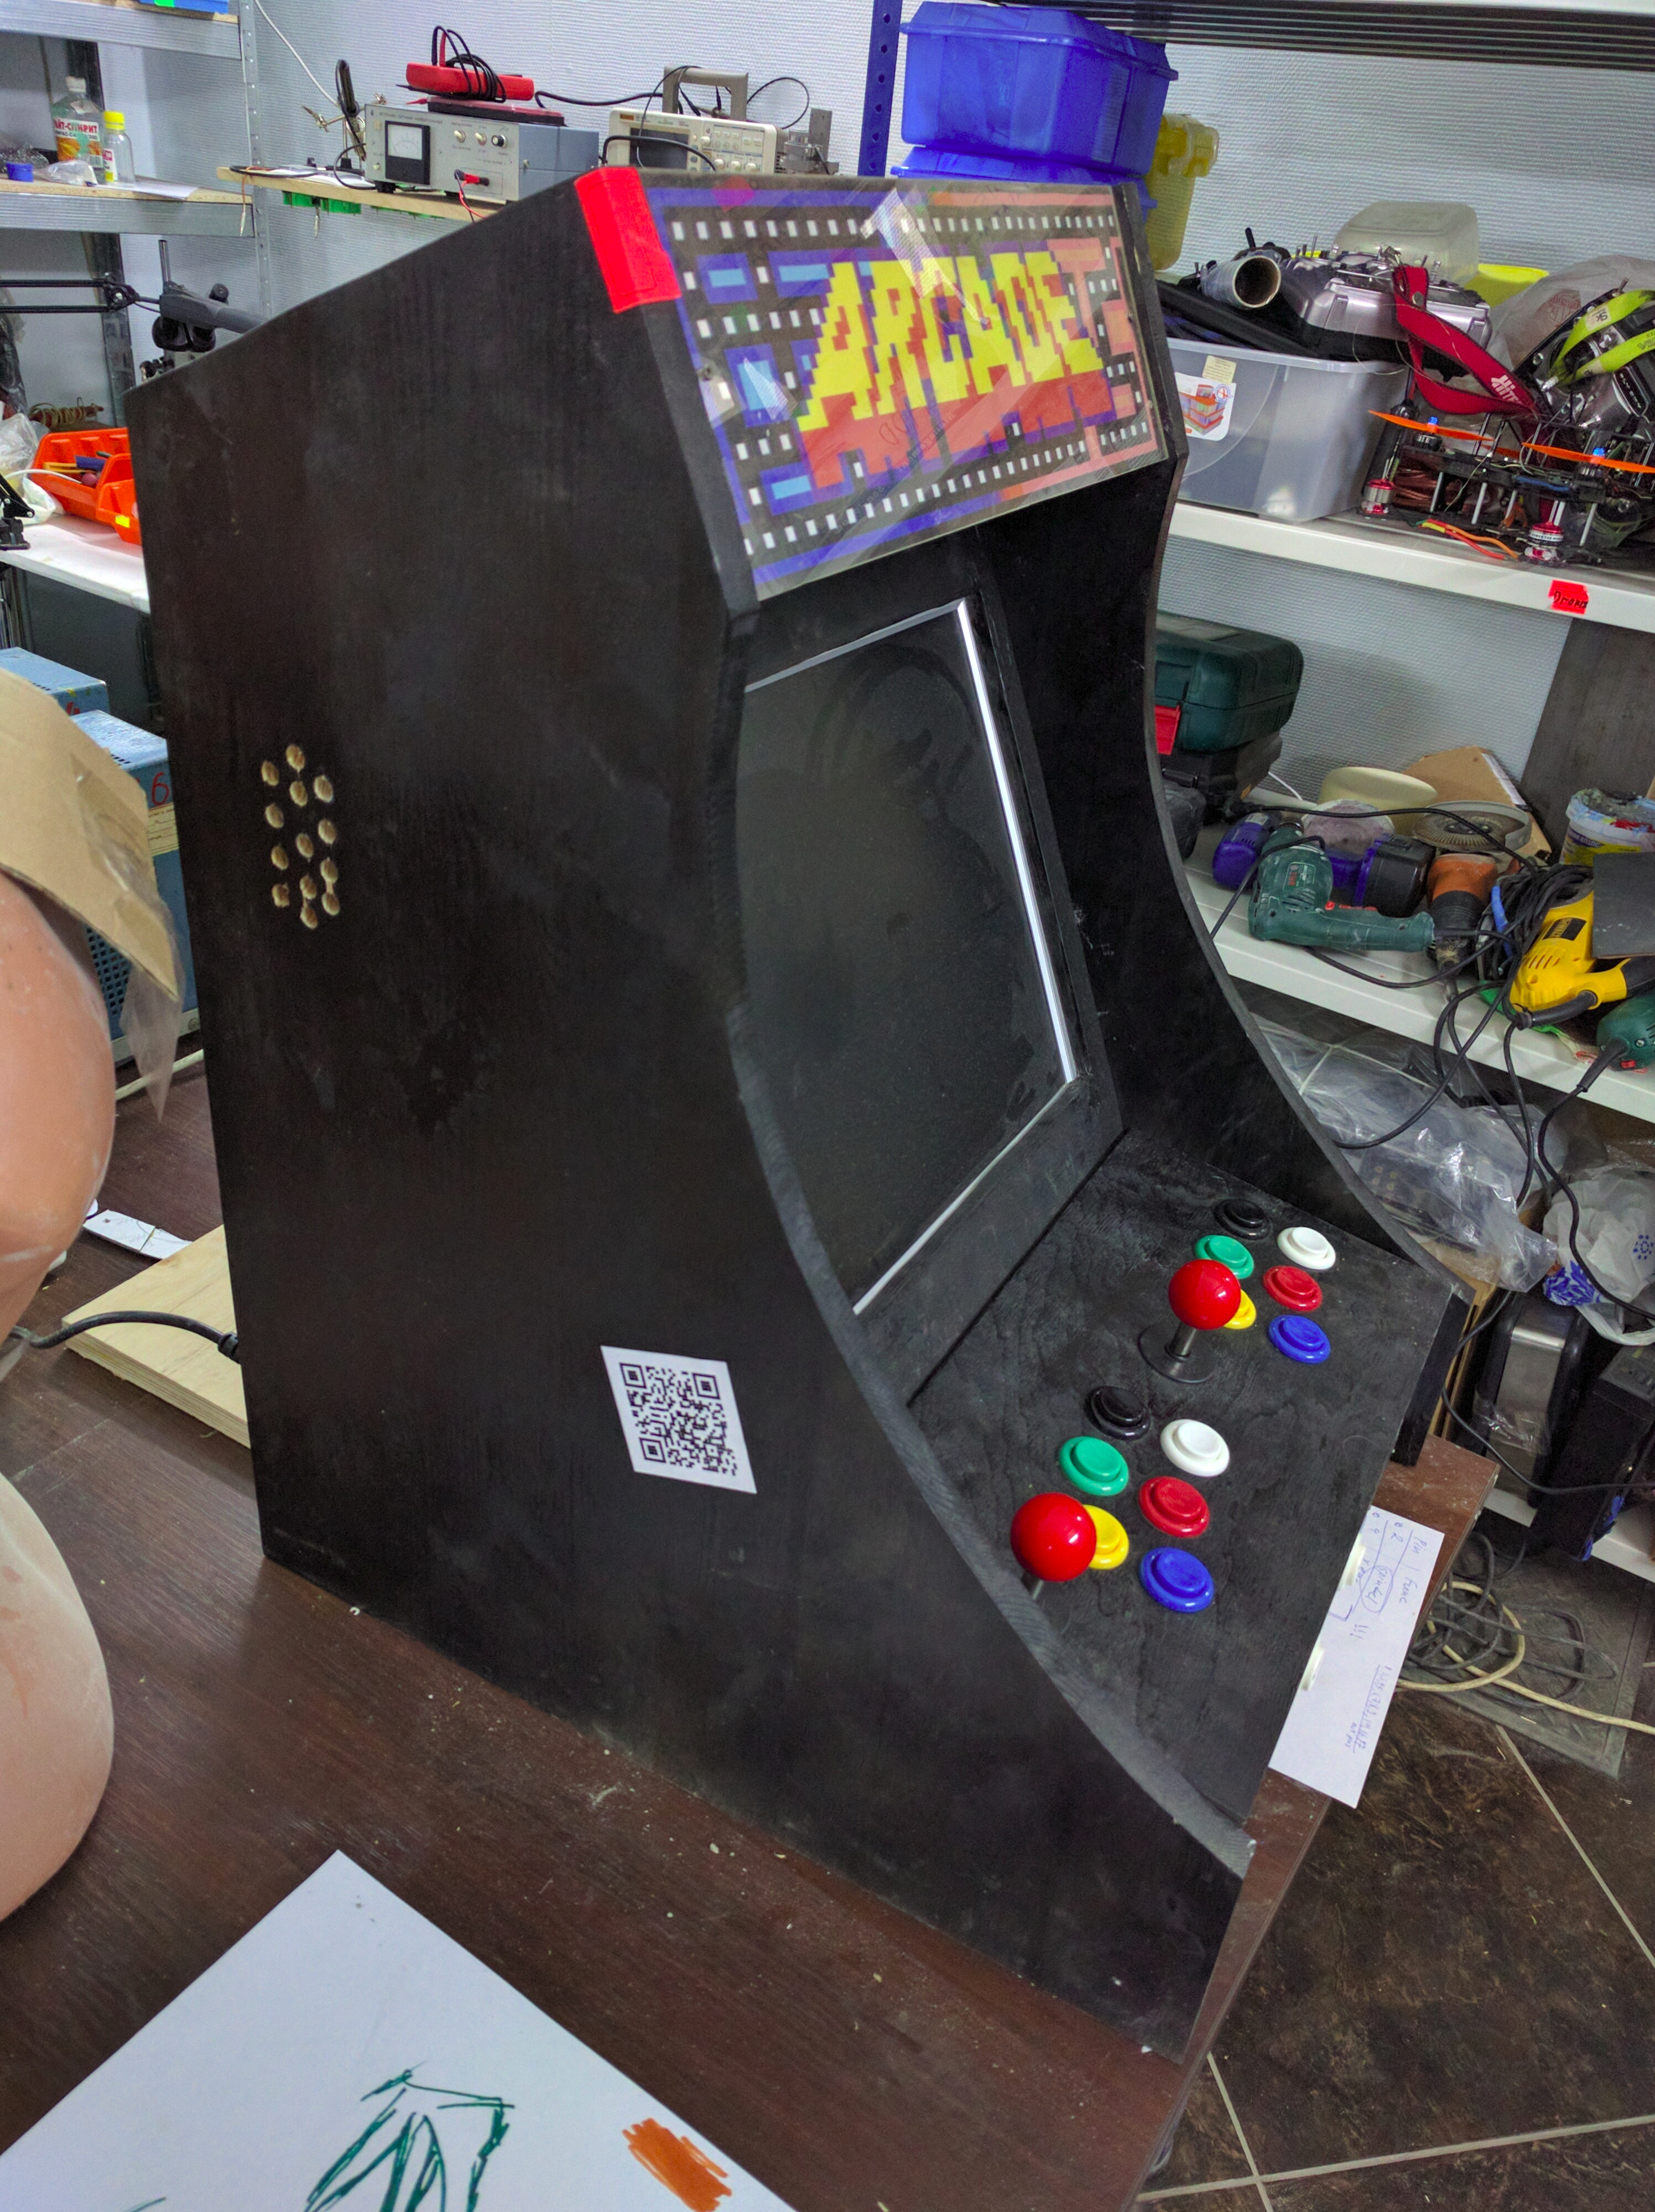
\includegraphics[height=5.7cm]{27_2016_Sorokin1.pdf}
\end{figure}

\subsection*{Работа над аппаратом. Программная часть}

Благодаря готовому дистрибутиву RetroPie настройка ПО прошла практически безболезненно. Но конечно не обошлось без загвоздок.
Потребовалось настраивать канал вывода звука (типовая проблема Pi), а также распознавание джойстиков, которые по умолчанию определялись как USB-мышь.

Дополнительного времени требует настройка M.A.M.E.: требуется скачивать BIOS-образы платформ,  а также конвертировать образы игр.
На этом же этапе обнаружилось, что количество реализованных в аппарате кнопок для многих игр M.A.M.E. маловато.

\begin{thebibliography}{99}
\bibitem{Sorokin1}Фронтэнд FB Alpha \url{http://www.fbalpha.com}
\bibitem{Sorokin2}Эмулятор M.A.M.E. \url{http://mamedev.org}
\bibitem{Sorokin3}Дистрибутив RetroPie \url{https://retropie.org.uk}
\bibitem{Sorokin4}Дистрибутив Lakka \url{http://www.lakka.tv}
\bibitem{Sorokin5}Фронтэнд RetroArch \url{http://www.libretro.com/index.php/retroarch-2/}
\bibitem{Sorokin6}Эмулятор LibRetro \url{http://www.libretro.com}
\bibitem{Sorokin7}САПР OpenScad \url{http://openscad.net}
\bibitem{Sorokin8}Образы ROM \url{https://duckduckgo.com/?q=arcade+roms}
\bibitem{Sorokin9}Описание проекта в персональном блоге  \url{http://alexsorokin.ru/retro-cabinet/}
\bibitem{Sorokin10}Опубликованные исходные коды \url{https://github.com/Gromina/bartop\_arcade}
\end{thebibliography}
\end{document}
